\documentclass[a4paper, 12pt]{article}
\usepackage{graphicx}
\usepackage{amsmath}
\usepackage{xcolor}
\usepackage{booktabs}
\usepackage[colorlinks = true,
linkcolor = blue,
urlcolor = blue,
citecolor = blue,
anchorcolor = blue]{hyperref}
\usepackage{longtable}
\usepackage{array}
% Elsevier/Data-in-Brief caption style: bold "Table N" label on its own
% line above the table; bold "Fig. N." label below the figure.
\usepackage{caption}
\captionsetup[table]{labelfont=bf,labelsep=newline,singlelinecheck=false,justification=raggedright,skip=4pt}
\captionsetup[figure]{name={Fig.},labelfont=bf,labelsep=period,skip=8pt}
\usepackage{fancyhdr}
\usepackage[headheight=2.6cm, top=1.3in, margin=1in]{geometry}
\renewcommand{\headrulewidth}{1pt}
% Data-in-Brief-style running banner (logo.png), generated by
% generate_banner.py. This is an original recreation of the journal
% template's colour/layout, not Elsevier's own trademarked logo artwork.
\fancyhead[L]{
\includegraphics[width=\textwidth]{logo.png}}
\fancyhead[R]{}
\renewcommand{\headrulewidth}{0pt}
\pagestyle{fancy}

\usepackage{fontspec}
% Set the main font to Carlito, matching the Data in Brief template.
% Falls back to TeX Gyre Termes if Carlito is unavailable (e.g. a fresh
% Overleaf project without the carlito font package installed).
\IfFontExistsTF{Carlito}{\setmainfont{Carlito}}{\setmainfont{TeX Gyre Termes}}
% Native Bengali script requires a Bengali-capable companion font.
\IfFontExistsTF{Nirmala UI}
  {\newfontfamily\bengalifont[Script=Bengali]{Nirmala UI}}
  {\IfFontExistsTF{Noto Serif Bengali}
    {\newfontfamily\bengalifont[Script=Bengali]{Noto Serif Bengali}}
    {\newfontfamily\bengalifont[Script=Bengali]{Noto Sans Bengali}}}
\newcommand{\bn}[1]{{\bengalifont #1}}

\usepackage[numbers,square]{natbib}
\bibliographystyle{elsarticle-num}
\usepackage{parskip}
\setlength{\parindent}{0pt}

\tolerance=1
\emergencystretch=\maxdimen
\hyphenpenalty=10000
\hbadness=10000

\usepackage{lineno}

% Auto-generated numeric macros, sourced from wsd_dataset.xlsx via
% analyze_dataset.py -> stats.json -> generate_tables.py -> numbers.tex
% AUTO-GENERATED by generate_tables.py -- do not hand-edit.
% Source of truth: stats.json, computed by analyze_dataset.py from wsd_dataset.xlsx
\newcommand{\NRows}{12059}
\newcommand{\NCols}{5}
\newcommand{\NWords}{402}
\newcommand{\NWordEntries}{421}
\newcommand{\NMultiEntryWords}{20}
\newcommand{\NSenseGlossStrings}{1085}
\newcommand{\NWordSensePairs}{1129}
\newcommand{\NWordIdSensePairs}{1205}
\newcommand{\SensesPerEntryMin}{2}
\newcommand{\SensesPerEntryMax}{4}
\newcommand{\SensesPerEntryMean}{2.86}
\newcommand{\ExPerWordMin}{1}
\newcommand{\ExPerWordMax}{120}
\newcommand{\ExPerWordMean}{30.00}
\newcommand{\ExPerClassMin}{9}
\newcommand{\ExPerClassMax}{20}
\newcommand{\ExPerClassMean}{10.01}
\newcommand{\RowsTargetNotInText}{874}
\newcommand{\MissingCells}{0}
\newcommand{\DupFullExtra}{0}
\newcommand{\DupTextExtra}{8}
\newcommand{\SentLenTokMin}{3}
\newcommand{\SentLenTokMax}{28}
\newcommand{\SentLenTokMean}{8.8}
\newcommand{\SentLenTokMedian}{7.0}
\newcommand{\SentLenTokStd}{4.2}
\newcommand{\SentLenCharMin}{13}
\newcommand{\SentLenCharMax}{165}
\newcommand{\SentLenCharMean}{54.1}


\begin{document}

\renewcommand{\linenumberfont}{\normalfont\normalsize}
\linenumbers

\section*{ARTICLE INFORMATION}

\subsection*{Article title}
A Sense-Annotated Dataset for Bangla Word Sense Disambiguation

\subsection*{Authors}
Prova Rani Paul\textsuperscript{a}, K. M. Azharul Hasan\textsuperscript{a,*}

\subsection*{Affiliations}
\textsuperscript{a}Department of Computer Science and Engineering, Khulna University of Engineering \& Technology (KUET), Khulna-9203, Bangladesh

\subsection*{Corresponding author's email address and Twitter handle}
az@cse.kuet.ac.bd (K. M. Azharul Hasan). \\
Prova Rani Paul's institutional email address: \textbf{[TO BE CONFIRMED]}. \\
Twitter/X handle: \textbf{[TO BE CONFIRMED]} (not available in source materials).

\subsection*{Keywords}
natural language processing; polysemy; corpus annotation; low-resource languages; inter-annotator agreement; lexical-sample corpus; contextual meaning classification

\subsection*{Abstract}
This article describes a sense-annotated dataset for Bangla (Bengali) Word Sense Disambiguation (WSD), released as a single structured spreadsheet, \texttt{wsd\_dataset.xlsx}. The file contains \NRows{} example sentences covering \NWords{} ambiguous Bangla target words (\NWordEntries{} independent word entries, since \NMultiEntryWords{} target words are represented by more than one separate sense inventory) and \NSenseGlossStrings{} distinct sense glosses. Each row records five fields: a numeric \texttt{word\_id}, the \texttt{target\_word} surface form, a \texttt{sense\_id}, a short Bangla \texttt{sense\_gloss}, and the example sentence (\texttt{text}) in which the target word is used in that sense.

Ambiguous target words were selected in two stages: 100 words were adopted from a previously published, public Bengali WSD word list, and 302 words were newly compiled for this work. For every word, candidate senses were validated against the \emph{Samsad Bangla Abhidhan} reference dictionary, and example sentences were then compiled for each word-sense pair from openly available Bangla reference material together with annotator-composed examples. Every sentence was subsequently labelled independently by two human annotators using a purpose-built PHP/MySQL web annotation platform that presents candidate senses in randomized order and enforces, through a database constraint, exactly one label per annotator per sentence. Annotation reliability was quantified with Cohen's kappa, computed per annotator against the platform's reference senses (0.836 and 0.874), corresponding to ``almost perfect'' agreement on the Landis--Koch scale.

The released file preserves the corpus exactly as annotated: it contains no missing values, and only \DupTextExtra{} duplicate example-sentence values across \NRows{} rows. This article reports the exact column-level schema, per-word and per-class distributions, sentence-length statistics, and a small character-encoding inconsistency discovered during verification (affecting two rows), so that downstream users can reuse, filter, or further clean the corpus with full transparency. The dataset is directly reusable for supervised WSD model training and evaluation, for benchmarking monolingual and multilingual language models on a genuinely polysemous low-resource language, and for broader Bangla natural language processing and corpus-annotation-reliability research.

\section*{SPECIFICATIONS TABLE}

% Per the official Data in Brief template, the Specifications Table is an
% unnumbered longtable; numbered tables start at Table 1 afterwards.
\begin{longtable}{| >{\raggedright\arraybackslash}p{3.4cm} | >{\raggedright\arraybackslash}p{10.8cm} |}
\hline
\textbf{Subject} & Computer Science \\
\hline
\textbf{Specific subject area} & Natural language processing; Bangla word sense disambiguation; sense-annotated lexical-sample corpus \\
\hline
\textbf{Type of data} & Table (single Microsoft Excel \texttt{.xlsx} file, \NCols{} columns, \NRows{} rows) \newline Raw, human-annotated \\
\hline
\textbf{Data collection} & \NWords{} ambiguous Bangla target words were selected (100 adopted from a prior public word list, 302 newly compiled). Candidate senses for every word were validated against the \emph{Samsad Bangla Abhidhan} dictionary. Example sentences were compiled per word-sense pair from openly available Bangla reference material and annotator-composed examples. Two independent annotators then labelled every sentence on a custom PHP/MySQL web platform (randomized sense order, SHA-256 import deduplication, one label per annotator per sentence enforced by a database constraint). Annotation reliability was measured with Cohen's kappa (0.836, 0.874). \\
\hline
\textbf{Data source location} & Department of Computer Science and Engineering, Khulna University of Engineering \& Technology (KUET), Khulna, Bangladesh \\
\hline
\textbf{Data accessibility} & % PLACEHOLDER: URL must be live and anonymously accessible at submission
Repository name: \textbf{[PUBLIC DATA REPOSITORY / DOI TO BE ADDED BEFORE SUBMISSION]} \newline
Data identification number: \textbf{[TO BE CONFIRMED]} \newline
Direct URL to data: \textbf{[TO BE CONFIRMED]} \newline
Instructions for accessing these data: The dataset must be deposited in a public repository (e.g. Mendeley Data, Zenodo, or Kaggle) prior to submission; this field is a placeholder until that deposit is complete. Dataset citation: \cite{bangla_wsd_dataset}. \\
\hline
\textbf{Related research article} & P. R. Paul and K. M. A. Hasan, ``Bangla Word Sense Disambiguation: A Large-Scale Benchmark of Embedding and Classifier Combinations,'' manuscript (publication venue and DOI \textbf{[TO BE CONFIRMED]}) \cite{paulhasan2025banglawsdbenchmark}. \\
\hline
\end{longtable}
\setcounter{table}{0} % Specifications Table is unnumbered; content tables start at Table 1

\section*{VALUE OF THE DATA}
\begin{itemize}
\item The related benchmark article reports this corpus as the largest published Bangla WSD dataset to date, based on a direct comparison against five previously published Bangla WSD studies covering 7--100 target words and 160--3,860 sentences; this release makes the full \NRows{}-row, \NWords{}-word corpus behind that comparison directly inspectable and reusable rather than summarized only as aggregate statistics in a page-limited conference paper.
\item Unlike every prior Bangla WSD dataset reviewed in the related article, this corpus reports a quantified inter-annotator reliability statistic (Cohen's kappa of 0.836 and 0.874), so other researchers can assess label trustworthiness directly rather than assuming it.
\item The flat five-column schema (\texttt{word\_id}, \texttt{target\_word}, \texttt{sense\_id}, \texttt{sense\_gloss}, \texttt{text}) requires no specialised parser and loads directly into pandas, R, or a spreadsheet application, lowering the barrier to reuse for supervised classification, few-shot evaluation, or contextual-embedding probing tasks.
\item Because every target word carries two to four dictionary-validated senses with genuine example sentences, the dataset is a realistic test bed for evaluating whether monolingual and multilingual transformer models (e.g. BanglaBERT \cite{bhattacharjee2022banglabert}, mBERT \cite{devlin2019bert}, XLM-R \cite{conneau2020xlmr}) actually encode sense-distinguishing context, rather than only word identity.
\item The dataset can be reused beyond WSD proper: as a resource for Bangla lexicography (dictionary-sense coverage checking), for studying annotator agreement methodology in low-resource-language corpus construction, and as training or evaluation data for Bangla sentence classification pipelines more generally.
\item The article's own quality analysis (missing-value check, duplicate check, verbatim target-word presence check, and a discovered character-encoding anomaly in two rows) is published alongside the data, so reuse decisions can be made with full knowledge of the corpus's actual, verified condition rather than an idealised description of it.
\end{itemize}

\section*{BACKGROUND}
Word Sense Disambiguation (WSD) -- selecting the correct meaning of an ambiguous word from context -- has historically relied, for Bangla, on small private datasets and hand-engineered features, with no dataset reporting a quantified annotation-reliability statistic. The related research article \cite{paulhasan2025banglawsdbenchmark} used this corpus to build a 29-experiment benchmark spanning lexical, static-embedding, recurrent, and transformer models, and reports that fine-tuned BanglaBERT reaches 89.72\% test accuracy on a word-specific-label formulation derived from this data. That article's page budget left no room to describe the released corpus itself in the depth a reuser needs: the exact column schema, the full distribution of senses and examples per word, sentence-length statistics, or a systematic data-quality check. This Data in Brief article addresses that gap: it describes the corpus exactly as released, independent of any particular downstream modeling choice, so that other researchers can verify its structure, assess its quality, and reuse it for tasks beyond the specific benchmark already published.

\section*{DATA DESCRIPTION}
The dataset is released as a single file, \texttt{wsd\_dataset.xlsx}, containing one worksheet with a single header row followed by \NRows{} data rows and \NCols{} columns. There are no merged cells, multi-row headers, or nested tables. Table~\ref{tab:schema} describes each column.

\begin{table}[htbp]
\caption{Column schema of \texttt{wsd\_dataset.xlsx}. All five columns are fully populated in every row.}
\label{tab:schema}
\centering
\small
\renewcommand{\arraystretch}{1.25}
\begin{tabular}{@{}p{2.4cm}p{2cm}p{9.9cm}@{}}
\toprule
\textbf{Column} & \textbf{Type} & \textbf{Description} \\
\midrule
\texttt{word\_id} & integer & Identifier for a \emph{word entry}, i.e. one target word together with one specific candidate-sense inventory. \NWordEntries{} distinct values exist across \NWords{} unique \texttt{target\_word} strings, because \NMultiEntryWords{} target words are each represented by more than one independent sense inventory (entered as separate \texttt{word\_id} values). \\
\addlinespace
\texttt{target\_word} & text (Bangla) & The ambiguous surface word being disambiguated in that row, e.g. \bn{জল}. \NWords{} unique strings occur in the file. \\
\addlinespace
\texttt{sense\_id} & integer & A small integer (observed range \SensesPerEntryMin{}--\SensesPerEntryMax{}) identifying one candidate sense within the \texttt{word\_id}'s sense inventory. \texttt{sense\_id} is scoped to its \texttt{word\_id}, not global: two different word entries may both contain a row with \texttt{sense\_id}~=~1, referring to unrelated senses. \\
\addlinespace
\texttt{sense\_gloss} & text (Bangla) & A short Bangla gloss naming the sense denoted by \texttt{sense\_id}, dictionary-validated (see Experimental Design). \NSenseGlossStrings{} unique gloss strings occur in the file; because glosses are short common Bangla words, a small number of gloss strings are shared verbatim by unrelated \texttt{word\_id} values, so \texttt{sense\_gloss} alone is not a unique class key (see \texttt{word\_id} above). \\
\addlinespace
\texttt{text} & text (Bangla) & The example sentence, written to contain the \texttt{target\_word} used specifically in the sense named by \texttt{sense\_gloss}. \\
\bottomrule
\end{tabular}
\end{table}

\subsection*{Dataset construction workflow}
Figure~\ref{fig:workflow} summarises the pipeline that produced the released file, from target-word selection through to the final structured spreadsheet; each stage is detailed in Experimental Design, Materials and Methods.

\begin{figure}[htbp]
\centering
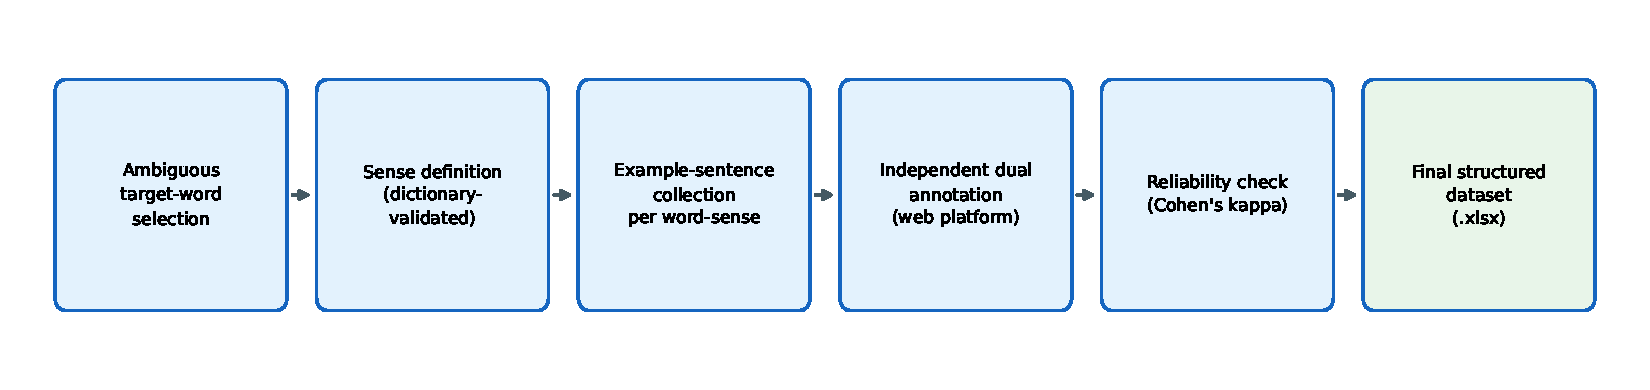
\includegraphics[width=\textwidth]{Figure_1_workflow.pdf}
\caption{Construction pipeline for the released dataset.}
\label{fig:workflow}
\end{figure}

\subsection*{Word- and sense-level structure}
Figure~\ref{fig:worddist} summarises the file at the word-entry level. Panel (a) shows that word entries carry 2 to 4 candidate senses each (\SensesPerEntryMin{}--\SensesPerEntryMax{}, mean \SensesPerEntryMean{}): 202 word entries have 2 senses, 75 have 3, and 144 have 4. Panel (b) shows the number of example sentences authored per \emph{unique target-word string} (\ExPerWordMin{}--\ExPerWordMax{}, mean \ExPerWordMean{}); the distribution clusters tightly around multiples of ten (20, 30, 40, 80, 120), consistent with roughly ten sentences having been collected per candidate sense. The two target words with only one example sentence are the character-encoding anomaly discussed under Limitations, not a genuine single-example word.

\begin{figure}[htbp]
\centering
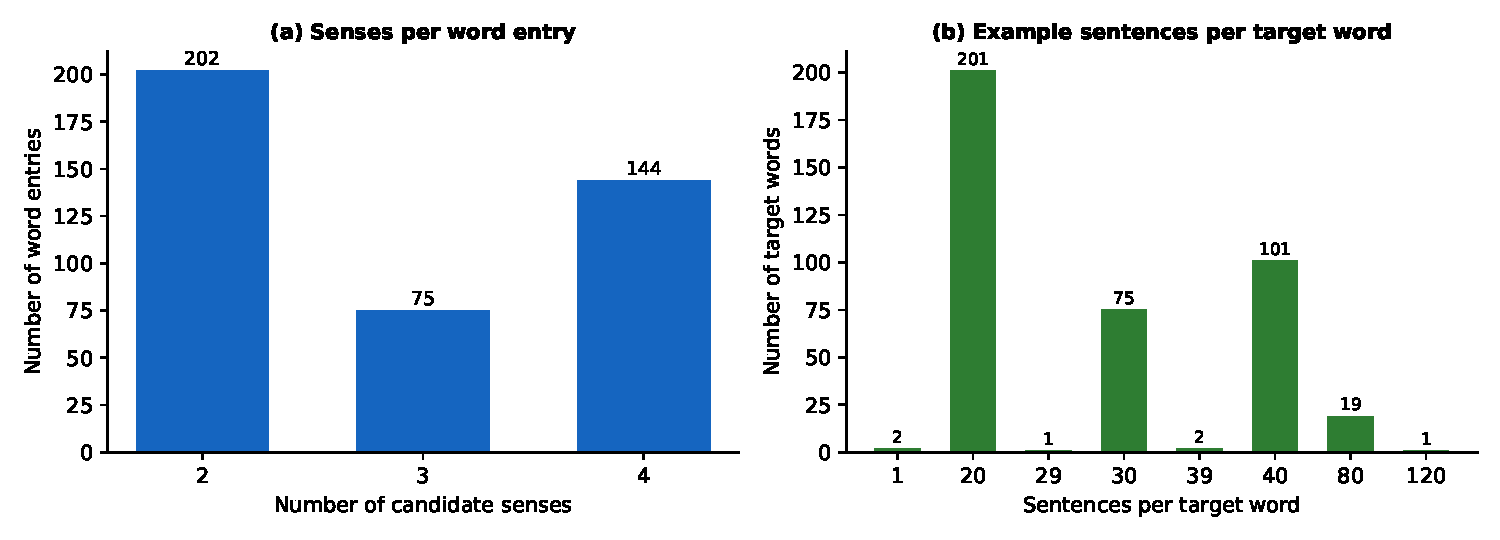
\includegraphics[width=\textwidth]{Figure_2_word_distributions.pdf}
\caption{(a) Number of candidate senses per word entry (\NWordEntries{} word entries). (b) Number of example sentences per unique \texttt{target\_word} string (\NWords{} target words).}
\label{fig:worddist}
\end{figure}

\subsection*{Example sentences per word-sense class}
Treating each (\texttt{word\_id}, \texttt{sense\_id}) pair as one class, the file contains \NWordIdSensePairs{} distinct word-sense classes, each holding \ExPerClassMin{} to \ExPerClassMax{} example sentences (mean \ExPerClassMean{}; Figure~\ref{fig:classsizes}). All but two classes hold exactly ten example sentences, reflecting a deliberate ten-sentences-per-sense collection target.

\begin{figure}[htbp]
\centering
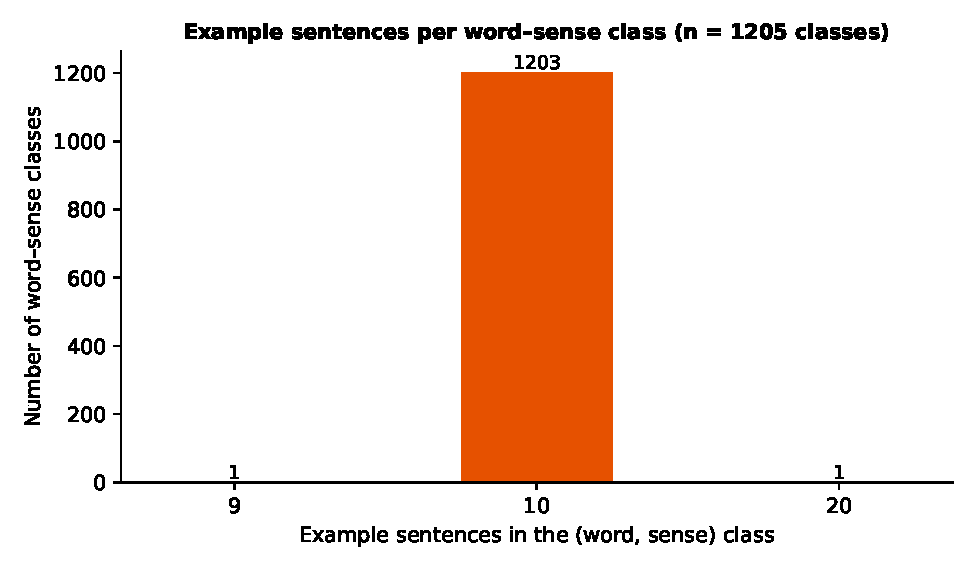
\includegraphics[width=0.72\textwidth]{Figure_3_class_sizes.pdf}
\caption{Number of example sentences per (\texttt{word\_id}, \texttt{sense\_id}) class.}
\label{fig:classsizes}
\end{figure}

\subsection*{Sentence-length distribution}
Sentence length, measured in whitespace-separated tokens, ranges from \SentLenTokMin{} to \SentLenTokMax{} tokens (mean \SentLenTokMean{}, median \SentLenTokMedian{}, standard deviation \SentLenTokStd{}); in characters, sentences range from \SentLenCharMin{} to \SentLenCharMax{} characters (mean \SentLenCharMean{}). Figure~\ref{fig:sentlen} shows the full token-length distribution, which is concentrated in the five-to-nine-token range and consistent with short, single-clause example sentences.

\begin{figure}[htbp]
\centering
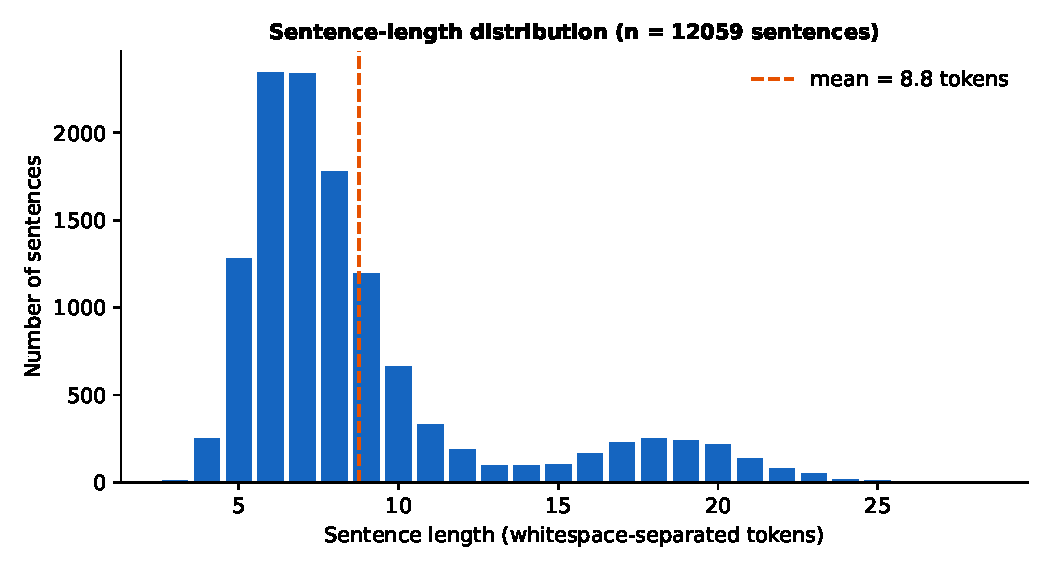
\includegraphics[width=0.72\textwidth]{Figure_4_sentence_length.pdf}
\caption{Sentence-length distribution across all \NRows{} example sentences (whitespace-separated tokens).}
\label{fig:sentlen}
\end{figure}

\subsection*{Dataset statistics overview}
Table~\ref{tab:stats} summarises the quantities computed directly from \texttt{wsd\_dataset.xlsx} by the accompanying \texttt{analyze\_dataset.py} script (see Experimental Design, Materials and Methods).

\begin{table}[htbp]
\caption{Quantitative overview of \texttt{wsd\_dataset.xlsx}, computed directly from the file.}
\label{tab:stats}
\centering
\small
\renewcommand{\arraystretch}{1.2}
\begin{tabular}{@{}lr@{}}
\toprule
\textbf{Attribute} & \textbf{Value} \\
\midrule
\multicolumn{2}{@{}l}{\textit{Corpus size}} \\
\quad Total example sentences (rows) & \NRows{} \\
\quad Columns & \NCols{} \\
\addlinespace
\multicolumn{2}{@{}l}{\textit{Word- and sense-level structure}} \\
\quad Unique \texttt{target\_word} strings & \NWords{} \\
\quad Unique \texttt{word\_id} (word entries) & \NWordEntries{} \\
\quad Target words with $>1$ word entry & \NMultiEntryWords{} \\
\quad Unique \texttt{sense\_gloss} strings & \NSenseGlossStrings{} \\
\quad Unique (\texttt{target\_word}, \texttt{sense\_gloss}) pairs & \NWordSensePairs{} \\
\quad Unique (\texttt{word\_id}, \texttt{sense\_id}) classes & \NWordIdSensePairs{} \\
\quad Senses per word entry (min / mean / max) & \SensesPerEntryMin{} / \SensesPerEntryMean{} / \SensesPerEntryMax{} \\
\quad Example sentences per target word (min / mean / max) & \ExPerWordMin{} / \ExPerWordMean{} / \ExPerWordMax{} \\
\quad Example sentences per word-sense class (min / mean / max) & \ExPerClassMin{} / \ExPerClassMean{} / \ExPerClassMax{} \\
\addlinespace
\multicolumn{2}{@{}l}{\textit{Sentence length}} \\
\quad In tokens (min / mean / max) & \SentLenTokMin{} / \SentLenTokMean{} / \SentLenTokMax{} \\
\quad In characters (min / mean / max) & \SentLenCharMin{} / \SentLenCharMean{} / \SentLenCharMax{} \\
\addlinespace
\multicolumn{2}{@{}l}{\textit{Integrity checks}} \\
\quad Missing cells (any column) & \MissingCells{} \\
\quad Fully duplicate rows (extra copies) & \DupFullExtra{} \\
\quad Rows with a duplicate \texttt{text} value (extra copies) & \DupTextExtra{} \\
\quad Rows where \texttt{target\_word} is absent from \texttt{text} & \RowsTargetNotInText{} \\
\bottomrule
\end{tabular}
\end{table}

\subsection*{Sample rows}
Table~\ref{tab:sample} shows six real rows for the target word \bn{জল} (\emph{jol}), illustrating three of its senses -- \bn{অত্যাধিক পরিশ্রম} (extreme toil), \bn{বৃষ্টি} (rain), and \bn{অশ্রু} (tears) -- with two example sentences each, exactly as they appear in the released file.

% AUTO-GENERATED by generate_tables.py -- real rows from wsd_dataset.xlsx, target_word = \bn{জল}
\begin{table}[htbp]
\caption{Sample rows from the released dataset for the target word \bn{জল} (\emph{jol}), illustrating three distinct senses of the same surface form, exactly as they appear in \texttt{wsd\_dataset.xlsx}.}
\label{tab:sample}
\centering
\footnotesize
\setlength{\tabcolsep}{4pt}
\renewcommand{\arraystretch}{1.3}
\begin{tabular}{@{}p{1.4cm}p{2.1cm}p{1.6cm}p{2.5cm}p{6.9cm}@{}}
\toprule
\texttt{word\_id} & \texttt{target\_word} & \texttt{sense\_id} & \texttt{sense\_gloss} & \texttt{text} \\
\midrule
1 & \bn{জল} & 1 & \bn{অত্যাধিক পরিশ্রম} & \bn{মাঠে সারাদিন রক্ত জল করা পরিশ্রম করেও কৃষক ন্যায্য মূল্য থেকে বঞ্চিত হন।} \\
1 & \bn{জল} & 1 & \bn{অত্যাধিক পরিশ্রম} & \bn{বছরের পর বছর রক্ত জল করা পরিশ্রম করে তিনি এই কারখানাটি দাঁড় করিয়েছেন।} \\
1 & \bn{জল} & 2 & \bn{বৃষ্টি} & \bn{আকাশভরা কালো মেঘ দেখে মনে হচ্ছে আজ প্রচণ্ড জল পড়বে।} \\
1 & \bn{জল} & 2 & \bn{বৃষ্টি} & \bn{কৃষকরা জল পড়ার অপেক্ষায় আকাশের দিকে তাকিয়ে আছেন কারণ ফসলের মাঠ শুকিয়ে গেছে।} \\
1 & \bn{জল} & 3 & \bn{অশ্রু} & \bn{সন্তানের বিদেশযাত্রার দিন মা চোখের জল আর আটকে রাখতে পারলেন না।} \\
1 & \bn{জল} & 3 & \bn{অশ্রু} & \bn{প্রিয় বন্ধুর মৃত্যুসংবাদ শুনে তার চোখ থেকে অনবরত জল পড়তে লাগল।} \\
\bottomrule
\end{tabular}
\end{table}


\section*{EXPERIMENTAL DESIGN, MATERIALS AND METHODS}

\subsection*{Target-word selection}
The target-word inventory was assembled in two stages. The first 100 ambiguous words were adopted from a previously published, publicly available Bengali WSD word list \cite{dasdawn2023}; the remaining 302 ambiguous words were newly compiled for this work, for a total of \NWords{} unique target-word strings.

\subsection*{Sense identification}
For every target word, candidate senses were defined as short Bangla glosses and validated against the \emph{Samsad Bangla Abhidhan} reference dictionary \cite{biswas2004sansad}. Each word entry (\texttt{word\_id}) carries between \SensesPerEntryMin{} and \SensesPerEntryMax{} candidate senses; 20 target words were re-entered with a second (or, for one word, a third) independent sense inventory, which is why the file contains \NWordEntries{} word entries over only \NWords{} unique target-word strings.

\subsection*{Sentence collection}
Example sentences were compiled for every word-sense pair from openly available Bangla reference material together with original, annotator-composed examples. The source materials available for this article do not identify a single named corpus, publication, or website as the origin of the sentence text, and this is reported here rather than inferred further.

\subsection*{Annotation}
Every sentence was subsequently checked independently by two human annotators on a purpose-built PHP/MySQL web annotation platform. The platform deduplicates imported sentences by a SHA-256 hash computed at import time, displays the candidate senses for each sentence's target word in randomized order to reduce positional bias, highlights the target word in the sentence, and enforces through a database constraint that a given annotator labels a given sentence only once. Sentences enter the platform only through an administrator-side bulk \texttt{.xlsx} import; the annotation interface itself only records sense selections and never edits sentence text. Annotation reliability was quantified with Cohen's kappa, computed per annotator against the platform's reference senses: $\kappa = 0.836$ and $\kappa = 0.874$, both ``almost perfect'' on the Landis--Koch scale \cite{cohen1960kappa,landis1977kappa}.

\subsection*{Data cleaning applied before this release}
The released file is the annotated corpus with minimal, transparent cleaning: rows are exactly as produced by the annotation platform's export, with duplicate import rows already removed by the platform's SHA-256 deduplication at import time. No rows have been removed for having an out-of-context target word, no rows have been merged across word entries, and no further filtering (such as removing rare sense classes) has been applied to this release. Consequently, and as reported transparently in Data Description and Limitations, \RowsTargetNotInText{} rows have a \texttt{target\_word} value that does not occur verbatim inside \texttt{text} (for example, due to inflectional suffixes attached to the target word in running text), and \DupTextExtra{} rows share an example-sentence value with another row for a different sense or word. Researchers who need a strictly verbatim-match or duplicate-free subset for a specific downstream task (e.g. the classification benchmark in the related research article \cite{paulhasan2025banglawsdbenchmark}, which applies exactly this filtering plus rare-class removal) should apply that filtering themselves from this raw release; the released file intentionally keeps that decision with the reuser rather than pre-applying it silently.

\subsection*{Dataset validation performed for this article}
For this article, the released file was validated programmatically (see Software and tools) by checking: column-level missing values; fully duplicate rows; duplicate \texttt{text} values; verbatim presence of \texttt{target\_word} inside \texttt{text}; the distribution of senses per word entry, example sentences per target word, and example sentences per word-sense class; and sentence-length statistics in tokens and characters. This check surfaced the character-encoding inconsistency reported in Limitations; no other structural anomaly was found, and no missing cells occur anywhere in the file.

\subsection*{Dataset formatting}
The released file is a single-sheet Microsoft Excel workbook (\texttt{.xlsx}) with a single header row and \NRows{} data rows, described column-by-column in Table~\ref{tab:schema}.

\subsection*{Software and tools}
Dataset analysis and figure generation for this article used Python 3.11 with pandas and openpyxl (\texttt{analyze\_dataset.py}, \texttt{generate\_tables.py}) and Matplotlib (\texttt{generate\_figures.py}), all included in the data repository alongside this manuscript's \LaTeX{} source. The annotation platform referenced above was implemented in PHP with a MySQL/MariaDB backend.

\section*{LIMITATIONS}
Two rows have a \texttt{target\_word} value containing a Latin letter (``\={\i}'', U+012B) in place of the correct Bangla vowel sign -- \bn{রান}\kern1.5pt\={\i} instead of \bn{রানী}, and \bn{নদ}\kern1.5pt\={\i} instead of \bn{নদী} -- while the corresponding \texttt{text} field is spelled correctly; this is a character-encoding artefact discovered during validation for this article, not a genuine additional target word, and it causes these two rows to appear as singleton target words in a naive per-string grouping. Separately, \RowsTargetNotInText{} rows have a \texttt{target\_word} that does not occur verbatim inside \texttt{text} (typically due to Bangla inflectional suffixes attached to the word in running text), and \DupTextExtra{} rows repeat an example-sentence value already used for another word or sense; neither has been filtered from this release (see Experimental Design). The precise origin of the example-sentence text is only partially documented in the source materials available for this article (``openly available Bangla reference material'' and ``annotator-composed examples''), without a named corpus or publication. The sense inventory reflects a single reference dictionary and was produced by two annotators rather than a larger annotator pool, so rare senses (as few as \ExPerClassMin{} example sentences) remain thinly supported for tasks that require many examples per class.

\section*{ETHICS STATEMENT}
This corpus was produced by two human annotators who gave informed consent and received a token honorarium for their work; they were free to skip any sentence they could not confidently label. No personal, sensitive, or identifying information about the annotators or any third party is stored in the released file: only the annotated sentence, the target word, and the selected sense are retained. The authors have read and followed the ethical requirements for publication in Data in Brief and confirm that this work does not involve human-subject experimentation beyond the compensated, consenting annotation task described above, does not involve animal experiments, and does not involve data collected from social media platforms.

\section*{CRediT AUTHOR STATEMENT}
\textbf{Prova Rani Paul:} Conceptualization, Data curation, Formal analysis, Investigation, Methodology, Software, Validation, Writing -- original draft. \textbf{K. M. Azharul Hasan:} Supervision, Validation, Writing -- review \& editing. \textit{These roles follow the single-author-thesis / supervisor structure documented in the authors' source materials and should be confirmed by the authors before submission} \textbf{[TO BE CONFIRMED BY AUTHORS]}.

\section*{ACKNOWLEDGEMENTS}
The authors thank the two annotators who labelled the corpus for their work, compensated with a token honorarium as described in the Ethics Statement. This research did not receive any specific grant from funding agencies in the public, commercial, or not-for-profit sectors.

\section*{DECLARATION OF COMPETING INTERESTS}
The authors declare that they have no known competing financial interests or personal relationships that could have appeared to influence the work reported in this paper.

\section*{REFERENCES}
\renewcommand{\refname}{}
\bibliography{references}

\end{document}
